
\documentclass[template=tabling,81pt,headonall]{azmoon}
\usepackage{xepersian}
\usepackage{amsfonts}
\usepackage{graphicx}
\usepackage{svg}
\svgpath{ {./images/} }
\graphicspath{ {./images/} }
\settextfont{Yas}
\setdigitfont{A Iranian Sans}
\usepackage{fontawesome5}

\printanswers
    \teacher{محمد صالح علی اکبری}
    \teachertitle{دبیر}
    \city{گناباد}
    \schooltitle{دبیرستان}
    \school{شهید جوانبخت}
    \grade{هفتم (نمونه ۱)}
    \branch{نمونه ۱}
    \topic{ریاضی}
    \examdate{۲۵ مهر ۱۴۰۵}
    \answertime{۳۵ دقیقه}
    \begin{document}
	\begin{questions}
		\nointerlineskip%
		\vskip-\baselineskip
		\question{%
یک ساختمان $5$ طبقه ساخته شده است. بالاترین طبقهٔ آن $2$ واحد دارد، اما هر یک طبقه که پایین می‌رویم، $2$ واحد به تعداد واحدها اضافه می‌شود.\\
الف) چه الگویی بین تعداد واحدها در طبقه‌های این ساختمان وجود دارد؟\\
ب) این ساختمان در کل چند واحد دارد؟‌
\\‌
\\‌
\\‌
\\}\question{%
قورباغه‌ای می‌خواهد از یک دیوار بالا برود. او با هر جهش $3$ متر بالا می‌رود و هر بار $2$ متر سُر می‌خورد و پایین می‌آید. اگر ارتفاع دیوار $9$ متر باشد، او با چند جهش به بالای دیوار می‌رسد؟ (رسم شکل یا نوشتن مراحل راه‌حل الزامی است)‌
\\‌
\\‌
\\‌
\\‌
\\‌
\\‌
\\}\question{%
با توجه به الگوی چوب‌کبریت‌های زیر:\\[0.3em]
\noindent
\begin{minipage}[c]{0.50\linewidth}
الف) شکل دهم با چند چوب‌کبریت ساخته می‌شود؟ \\\\[0.8em]
ب) چرا؟ (رابطه یا روش خود را توضیح دهید)
\end{minipage}\hfill
\begin{minipage}[c]{0.48\linewidth}
\centering
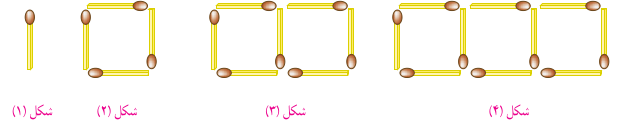
\includegraphics[width=\linewidth]{haftom_choob_kebrit}
\end{minipage}‌
\\‌
\\‌
\\‌
\\‌
\\}\end{questions}
    \end{document}
    